\documentclass{beamer}
\usepackage[outputdir=build]{minted}
\usepackage[skins,minted,breakable]{tcolorbox}
\usepackage[spanish]{babel}
\usepackage{subcaption}
\usetikzlibrary{matrix,backgrounds}
\usepackage{multirow}
\usepackage{multicol}
\usepackage{adjustbox}
\usepackage{soul}

\graphicspath{ {../img/} {../../LaTeX/img/} {/home/csp98/latex/img/}}
\selectlanguage{spanish}
\usepackage[utf8]{inputenc}
\usetheme{PaloAlto}
\setbeamerfont{section in sidebar}{size=\fontsize{2}{4}\selectfont}
\setbeamerfont{subsection in sidebar}{size=\fontsize{2}{3}\selectfont}
\setbeamerfont{subsubsection in sidebar}{size=\fontsize{2}{2}\selectfont}

\setbeamerfont{section in toc}{size=\footnotesize}
\setbeamerfont{subsection in toc}{size=\scriptsize}
\setbeamerfont{subsubsection in toc}{size=\tiny}

\usetikzlibrary{arrows,positioning,automata,shadows,fit,shapes,calc}



\title{Práctica 4}
\date{25 de mayo de 2018}
\subtitle{El viajante de comercio}

\author{María Jesús López Salmerón \\ Nazaret Román Guerrero \\ Laura Hernández Muñoz \\ José Baena Cobos  \\ Carlos Sánchez Páez}

\makeatletter
  \setbeamertemplate{sidebar \beamer@sidebarside}%{sidebar theme}
  {
    \beamer@tempdim=\beamer@sidebarwidth%
    \advance\beamer@tempdim by -6pt%
    \insertverticalnavigation{\beamer@sidebarwidth}%
    \vfill
    \ifx\beamer@sidebarside\beamer@lefttext%
    \else%
      \usebeamercolor{normal text}%
      \llap{\usebeamertemplate***{navigation symbols}\hskip0.1cm}%
      \vskip2pt%
    \fi%
}%
\makeatother

\subject{Algorítmica}
\AtBeginSection[]
  {
     \begin{frame}<beamer>
     \frametitle{Índice}
     \tableofcontents[currentsection]
     \end{frame}
  }
\AtBeginSubsection[]
{
  \begin{frame}<beamer>{Índice}
    \tableofcontents[currentsection,currentsubsection]
  \end{frame}
}
\AtBeginSubsubsection[]
{
  \begin{frame}<beamer>{Índice}
    \tableofcontents[currentsection,currentsubsection]
  \end{frame}
}

% Let's get started
\begin{document}
\centering
\begin{frame}
  \titlepage
\end{frame}

\begin{frame}{Índice}
  \tableofcontents
  % You might wish to add the option [pausesections]
\end{frame}

\section{Descripción del algoritmo}

\subsection{Estructuras utilizadas}
\begin{frame}[fragile]{Primeros pasos}
\begin{enumerate}
	\item<+-> \textbf{Estimador}.
	$\centering \frac{1}{2} \sum_{i=0}^{n}coste_{entrada}(i)+coste_{salida}(i)$
	\item<+-> \textbf{Camino}. Vector de ciudades. Almacena la solución final.
	\item<+-> \textbf{Solución parcial}. Vector de ciudades.
	\item<+-> \textbf{Mejor distancia}. Comienza siendo $+\infty$.
\end{enumerate}
\end{frame}
\subsection{Algoritmo paso a paso}

\begin{frame}[fragile]{Primeros pasos}

\begin{enumerate}
	\item<+-> Calculamos cota inferior mediante estimador.
	\item<+-> $s_{parcial}$ $\leftarrow$ ciudades[0].
	\item<+-> visitados[ciudades[0]]=true
	\item<+-> Llamamos al algoritmo recursivo.
\end{enumerate}
\end{frame}


\begin{frame}[fragile]{Algoritmo recursivo}

\begin{enumerate}
	\item<+-> \textbf{Caso base}: nodo hoja.
	\begin{enumerate}
		\item<+-> Si la solución parcial actual es mejor que la global, actualizamos.
	\end{enumerate}
	\item<+-> Para cada ciudad restante:
	\begin{enumerate}
		\item<+-> Si no ha sido visitada la añadimos al recorrido.
		\item<+-> Calculamos la cota de la rama actual.
		\item<+-> Si $cota_{actual} + distancia_{actual} < distancia_{mejor}$ expandimos  el nodo.
	\end{enumerate}
\end{enumerate}
\end{frame}


\section{Ejemplo}

\begin{frame}[fragile]{Ejemplo (3 ciudades)}
\large{
\[
  D=\begin{bmatrix}
    0 & 4 & 2 \\
    4 & 0 & 3 \\
    2 & 3 & 0 \\
  \end{bmatrix}
 \]
}
\end{frame}

\begin{frame}[fragile]{Ejemplo (3 ciudades)}
$
  D=\begin{bmatrix}
    0 & 4 & 2 \\
    4 & 0 & 3 \\
    2 & 3 & 0 \\
  \end{bmatrix}
$
 \begin{figure}[H]
\begin{tikzpicture}[sibling distance=10em,
  every node/.style = {shape=rectangle, rounded corners,
    draw, align=center,
    top color=white, bottom color=blue!20}]]
  \node[top color=green!30, bottom color=white] {1};
\end{tikzpicture}
\end{figure}
cota = estimador() =  9\\
Añadimos la ciudad 1 al camino.\\
$s_{parcial}=\{c_1\}$\\
$d_{mejor}=+\infty$
\end{frame}

\begin{frame}[fragile]{Ejemplo (3 ciudades)}
$
  D=\begin{bmatrix}
    0 & 4 & 2 \\
    4 & 0 & 3 \\
    2 & 3 & 0 \\
  \end{bmatrix}
$
 \begin{figure}[H]
\begin{tikzpicture}[sibling distance=10em,
  every node/.style = {shape=rectangle, rounded corners,
    draw, align=center,
    top color=white, bottom color=blue!20}]]
  \node[top color=green!30, bottom color=white] {1}
    child { 
    node {2}
    };
\end{tikzpicture}
\end{figure}
cota =  9\\
No es un nodo hoja $\rightarrow$ Calculamos su primer hijo.\\
$s_{parcial}=\{c_1\}$\\
$d_{mejor}=+\infty$
\end{frame}

\begin{frame}[fragile]{Ejemplo (3 ciudades)}
$
  D=\begin{bmatrix}
    0 & 4 & 2 \\
    4 & 0 & 3 \\
    2 & 3 & 0 \\
  \end{bmatrix}
$
 \begin{figure}[H]
\begin{tikzpicture}[sibling distance=10em,
  every node/.style = {shape=rectangle, rounded corners,
    draw, align=center,
    top color=white, bottom color=blue!20}]]
  \node[top color=green!30, bottom color=white] {1}
    child { 
    node[top color=green!30, bottom color=white] {2}
    };
\end{tikzpicture}
\end{figure}
cota  = 9 \\
No ha sido visitado $\rightarrow$ lo añadimos al camino.\\
$s_{parcial}=\{c_1,c_2\}$\\
$d_{mejor}=+\infty$
\end{frame}

\begin{frame}[fragile]{Ejemplo (3 ciudades)}
$
  D=\begin{bmatrix}
    0 & 4 & 2 \\
    4 & 0 & 3 \\
    2 & 3 & 0 \\
  \end{bmatrix}
$
 \begin{figure}[H]
\begin{tikzpicture}[sibling distance=10em,
  every node/.style = {shape=rectangle, rounded corners,
    draw, align=center,
    top color=white, bottom color=blue!20}]]
  \node[top color=green!30, bottom color=white] {1}
    child { 
    node {2}
    };
\end{tikzpicture}
\end{figure}
cota  = 9 \\
Calculamos nueva cota. nueva=2.5\\
$s_{parcial}=\{c_1,c_2\}$\\
$d_{mejor}=+\infty$
\end{frame}

\begin{frame}[fragile]{Ejemplo (3 ciudades)}
$
  D=\begin{bmatrix}
    0 & 4 & 2 \\
    4 & 0 & 3 \\
    2 & 3 & 0 \\
  \end{bmatrix}
$
 \begin{figure}[H]
\begin{tikzpicture}[sibling distance=10em,
  every node/.style = {shape=rectangle, rounded corners,
    draw, align=center,
    top color=white, bottom color=blue!20}]]
  \node[top color=green!30, bottom color=white] {1}
    child { 
    node {2}
    };
\end{tikzpicture}
\end{figure}
cota  = \textst{9} 2.5 \\
\textcolor{green}{Es mejor} $\rightarrow$ actualizo cota.
$s_{parcial}=\{c_1,c_2\}$\\
$d_{mejor}=+\infty$
\end{frame}

\begin{frame}[fragile]{Ejemplo (3 ciudades)}
$
  D=\begin{bmatrix}
    0 & 4 & 2 \\
    4 & 0 & 3 \\
    2 & 3 & 0 \\
  \end{bmatrix}
$
 \begin{figure}[H]
\begin{tikzpicture}[sibling distance=10em,
  every node/.style = {shape=rectangle, rounded corners,
    draw, align=center,
    top color=white, bottom color=blue!20}]]
  \node[top color=green!30, bottom color=white] {1}
    child { 
    node[top color=green!30, bottom color=white] {2}
    	child{
    		node{3}
    	}
    };
\end{tikzpicture}
\end{figure}
cota  = 2.5 \\
$cota + distancia_{actual}=6.5 < + \infty \rightarrow$ Exploro.\\
$s_{parcial}=\{c_1,c_2\}$\\
$d_{mejor}=+\infty$
\end{frame}

\begin{frame}[fragile]{Ejemplo (3 ciudades)}
$
  D=\begin{bmatrix}
    0 & 4 & 2 \\
    4 & 0 & 3 \\
    2 & 3 & 0 \\
  \end{bmatrix}
$
 \begin{figure}[H]
\begin{tikzpicture}[sibling distance=10em,
  every node/.style = {shape=rectangle, rounded corners,
    draw, align=center,
    top color=white, bottom color=blue!20}]]
  \node[top color=green!30, bottom color=white] {1}
    child { 
    node[top color=green!30, bottom color=white] {2}
    	child{
    		node[top color=green!30, bottom color=white]{3}
    	}
    };
\end{tikzpicture}
\end{figure}
cota  =  2.5 \\
Es nodo terminal y actualizo camino y distancia mejor.\\
$s_{parcial}=\{c_1,c_2,c_3,c_1\}$\\
$d_{mejor}$=\textst{$+\infty$}=9
\end{frame}

\begin{frame}[fragile]{Ejemplo (3 ciudades)}
$
  D=\begin{bmatrix}
    0 & 4 & 2 \\
    4 & 0 & 3 \\
    2 & 3 & 0 \\
  \end{bmatrix}
$
 \begin{figure}[H]
\begin{tikzpicture}[sibling distance=10em,
  every node/.style = {shape=rectangle, rounded corners,
    draw, align=center,
    top color=white, bottom color=blue!20}]]
  \node[top color=green!30, bottom color=white] {1}
    child { 
    node {2}
    	child{
    		node{3}
    	}
    }
    child { 
    	node {3}
    };
\end{tikzpicture}
\end{figure}
cota  =  2.5 \\
Vuelvo al nodo raíz y calculo su otro hijo.\\
$s_{parcial}=\{c_1\}$\\
$d_{mejor}=6$
\end{frame}

\begin{frame}[fragile]{Ejemplo (3 ciudades)}
$
  D=\begin{bmatrix}
    0 & 4 & 2 \\
    4 & 0 & 3 \\
    2 & 3 & 0 \\
  \end{bmatrix}
$
 \begin{figure}[H]
\begin{tikzpicture}[sibling distance=10em,
  every node/.style = {shape=rectangle, rounded corners,
    draw, align=center,
    top color=white, bottom color=blue!20}]]
  \node[top color=green!30, bottom color=white] {1}
    child { 
    node {2}
    	child{
    		node{3}
    	}
    }
    child { 
    	node[top color=green!30, bottom color=white] {3}
    };
\end{tikzpicture}
\end{figure}
cota  =  2.5 \\
No ha sido visitado $\rightarrow$ lo añadimos al camino.\\
Calculo la nueva cota. nueva=3.2 \\
$s_{parcial}=\{c_1,c_3\}$\\
$d_{mejor}=9$
\end{frame}

\begin{frame}[fragile]{Ejemplo (3 ciudades)}
$
  D=\begin{bmatrix}
    0 & 4 & 2 \\
    4 & 0 & 3 \\
    2 & 3 & 0 \\
  \end{bmatrix}
$
 \begin{figure}[H]
\begin{tikzpicture}[sibling distance=10em,
  every node/.style = {shape=rectangle, rounded corners,
    draw, align=center,
    top color=white, bottom color=blue!20}]]
  \node[top color=green!30, bottom color=white] {1}
    child { 
    node {2}
    	child{
    		node{3}
    	}
    }
    child { 
    	node[top color=red!30, bottom color=white] {3}
    };
\end{tikzpicture}
\end{figure}
cota  =  2.5 \\
Calculo la nueva cota. nueva=3.2 \\
Es mayor $\rightarrow$ no exploro.\\
$s_{parcial}=\{c_1,c_3\}$\\
$d_{mejor}=9$
\end{frame}




\section{Resultados obtenidos}

\begin{frame}[fragile]{uluysses6}
\begin{figure}[H]
\centering
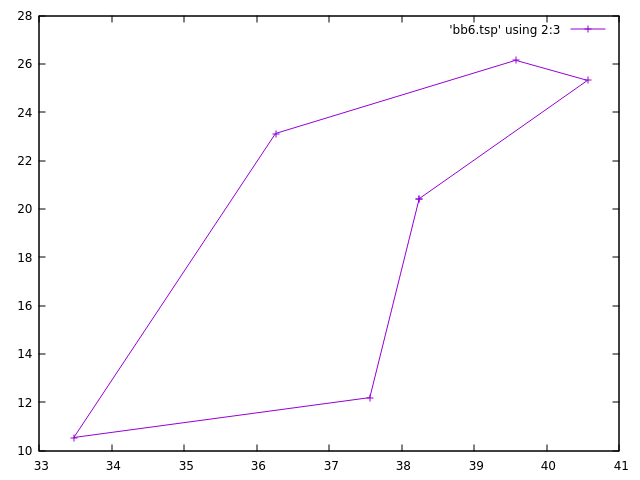
\includegraphics[scale=0.5]{bb6.png}
\end{figure}
\end{frame}

\begin{frame}[fragile]{uluysses7}
\begin{figure}[H]
\centering
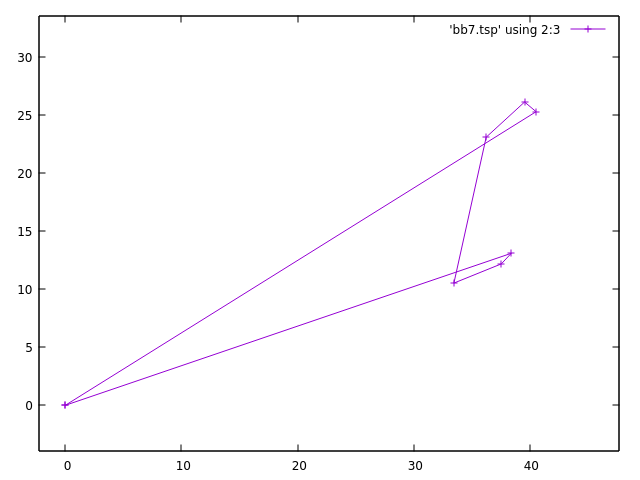
\includegraphics[scale=0.5]{bb7.png}
\end{figure}
\end{frame}

\begin{frame}[fragile]{uluysses8}
\begin{figure}[H]
\centering
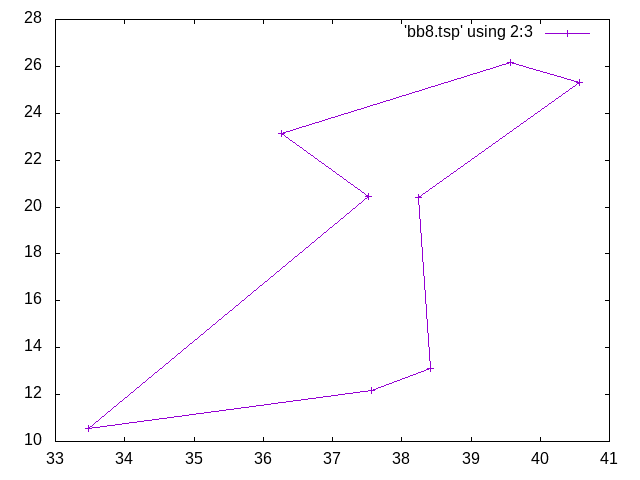
\includegraphics[scale=0.5]{bb8.png}
\end{figure}
\end{frame}

\begin{frame}[fragile]{uluysses9}
\begin{figure}[H]
\centering
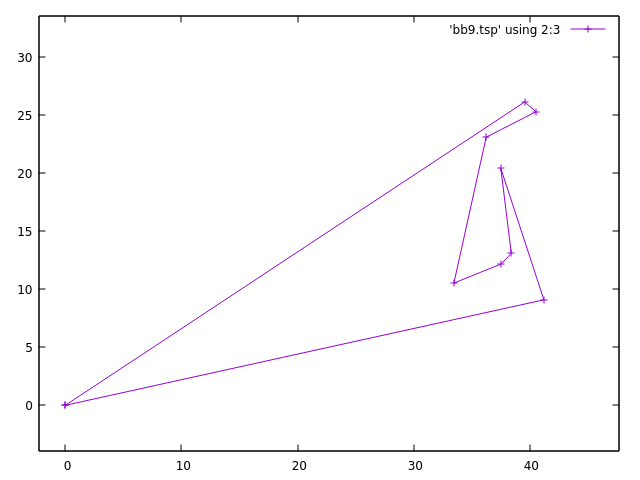
\includegraphics[scale=0.5]{bb9.png}
\end{figure}
\end{frame}

\begin{frame}[fragile]{uluysses10}
\begin{figure}[H]
\centering
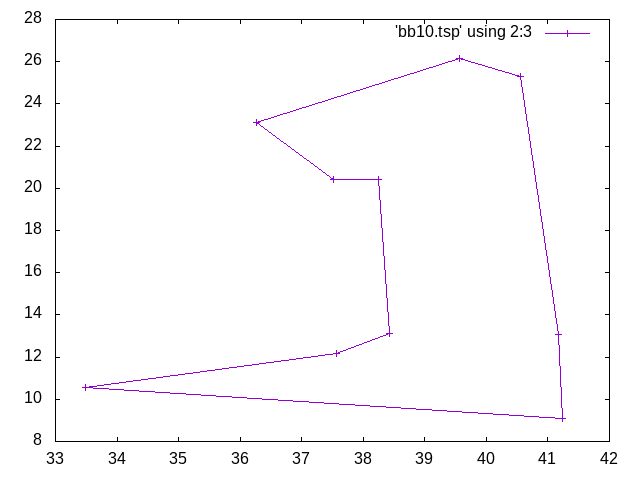
\includegraphics[scale=0.5]{bb10.png}
\end{figure}
\end{frame}

\begin{frame}[fragile]{uluysses11}
\begin{figure}[H]
\centering
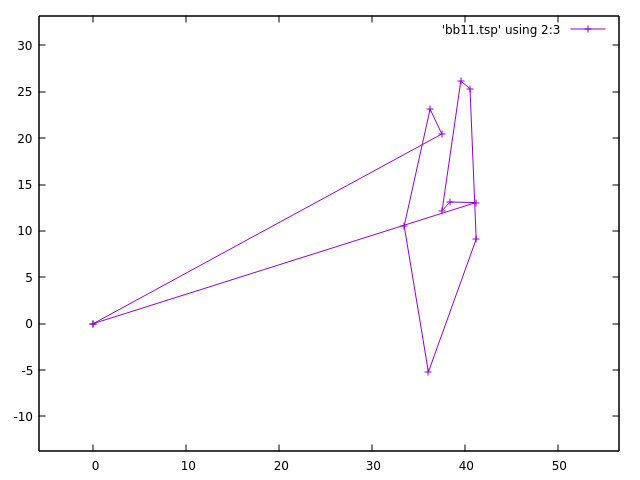
\includegraphics[scale=0.5]{bb11.png}
\end{figure}
\end{frame}

\begin{frame}[fragile]{uluysses12}
\begin{figure}[H]
\centering
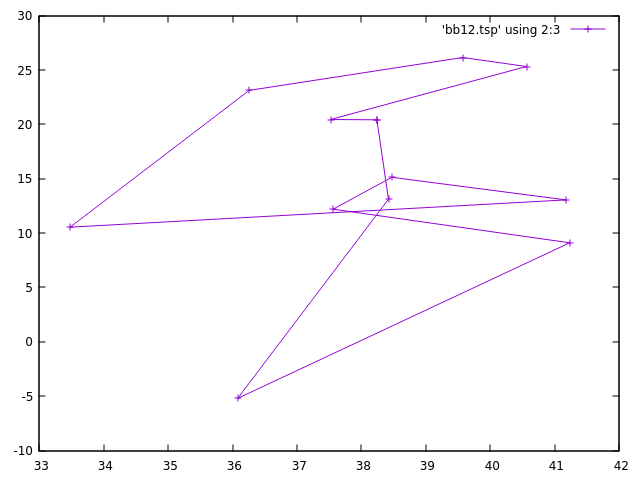
\includegraphics[scale=0.5]{bb12.png}
\end{figure}
\end{frame}

\begin{frame}[fragile]{uluysses13}
\begin{figure}[H]
\centering
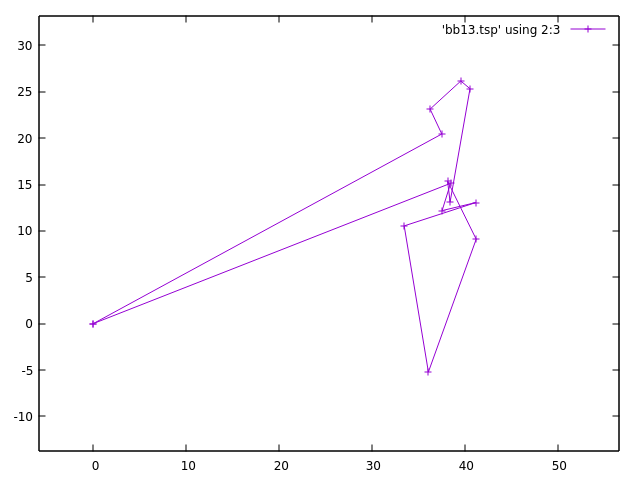
\includegraphics[scale=0.5]{bb13.png}
\end{figure}
\end{frame}

\begin{frame}[fragile]{uluysses14}
\begin{figure}[H]
\centering
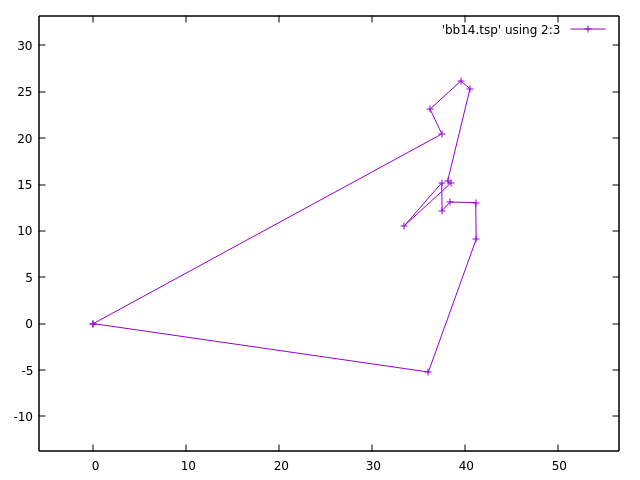
\includegraphics[scale=0.5]{bb14.png}
\end{figure}
\end{frame}

\begin{frame}[fragile]{uluysses15}
\begin{figure}[H]
\centering
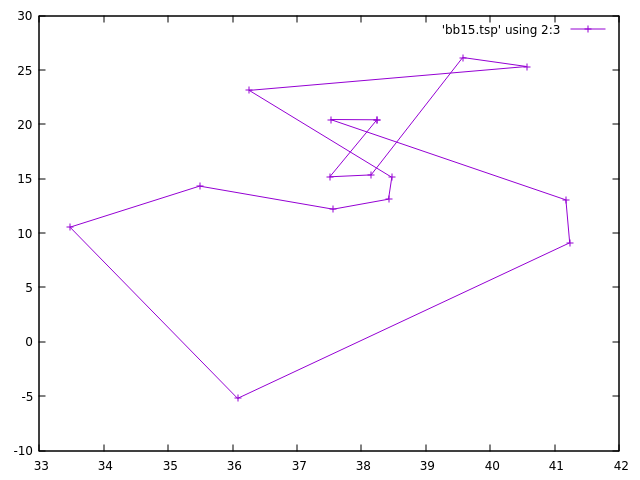
\includegraphics[scale=0.5]{bb15.png}
\end{figure}
\end{frame}

\begin{frame}[fragile]{Tiempos}
\begin{figure}[H]
\centering
\begin{tabular}{|c|c|}
\hline
\textbf{Número de ciudades} & \textbf{Tiempo(s)}\\
\hline
6 & $1.27 \cdot 10^{-5}$\\
\hline
7 & $4.39 \cdot 10^{-5}$\\
\hline
8 & $0.0002036$\\
\hline
9 & $0.0054381$\\
\hline
10 & $0.0325048$\\
\hline
11 & $0.381596$\\
\hline
12 & $2.23487$\\
\hline
13 & $8.90865$\\
\hline
14 & $107.772$ (2 minutos y 20 segundos)\\
\hline
15 & $1192.761$ (19 minutos y 53 segundos)\\
\hline
16 & $+4h$\\
\hline
\end{tabular}
\end{figure}
\end{frame}

\section*{Fin de la presentación}

\begin{frame}{Fin}
\begin{center}
\huge{Fin de la presentación}
\end{center}
\end{frame}


\end{document}


